% -*- mode: latex; mode: auto-fill; coding: utf-8; -*-

\chapter{Procedural generation of content}
\label{chap:noise}
What is known as procedural or synthetic generation of content is
used extensively in computer graphics to enable generation of natural
looking details. By generating details, in contrast to doing them by
hand, boring work typically done by computer artists can be cut down.
%and instead be used on designing the overall look and feel.
%
The term procedural generation of content is very fuzzy and covers
quite a large area of different techniques, but boils down to some
kind of algorithm that produces data \citebook{page~12}{ebert2003}.
The algorithm typically has a number of parameters that can be
specified to control the generation process in a way that alters the
result in an intuitive way based on the parameters.

\section{Generating irregular data}
We have chosen to concentrate our effort on irregular data generation
minded on textures, therefore only this type of data generation
will be covered in the following.
%
The basic building blocks when generating irregular data are
noise functions. A noise function is a function that is apparently
stochastic and will break up monotony of the patterns that would
otherwise be too regular \citebook{page~67-78}{ebert2003}.
%
Typically a noise function is a function of a position so the arguments
can be filled directly when rendering, e.g. $f(x,y,z)$.
%
An obvious stochastic primitive is uniformly distributed random
numbers with no correlation, which is also known as white noise.
In computer graphics however true random numbers are rarely used,
because they are not controllable.
Instead pseudo random number, PRN, generators are used to produce a
fair approximation to white noise. These however are controllable and
furthermore produce the same number sequences on two successive runs
provided the algorithm is started with the same preconditions.
%
Another property of white noise that we do not want is that it is
uncorrelated in all function values. This causes problems in computer
graphics because of rounding errors in the floating point
representation used when rendering. Instead we use a low-pass filtered
version of an approximation to white noise.

There are many different ways of using PRN to produce noise functions,
each method generates functions with different properties. Generally the
functions are divided into categories based on how they generate the
noise. To make an important and often misunderstood point regarding
what precisely defines the famous Perlin noise function, we will
introduce two basic categories of noise functions: Value and gradient
noise, which both also are categorized as lattice noise.

%\pagebreak

\subsection{Lattice noise}
In geometry a lattice is a discrete subgroup (a set of points) in the
same dimension as the basis vectors spanning the vector space. A
lattice can be viewed as a regular tiling of space by primitive cells
forming a grid structure. The most used lattice in computer graphics is the
regular Cartesian grid, which can be viewed as a tiling of
squares in two dimensions, see figure \ref{fig:square-lattice}. For
clarity figure \ref{fig:lattices} also provides other examples of
lattices.

\begin{figure}[!h]
  \centering
  \subfloat[Triangle lattice.]{
    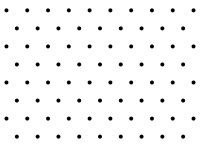
\includegraphics[width=3cm]{200px-Equilateral_Triangle_Lattice}
    \label{fig:lattice1}
  }
  \hspace{4mm}
  \subfloat[Rhombic lattice.]{
    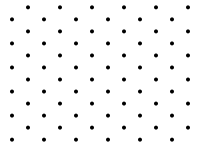
\includegraphics[width=3cm]{200px-Rhombic_Lattice}
    \label{fig:lattice2}
  }
  \hspace{4mm}
  \subfloat[Square lattice.]{
    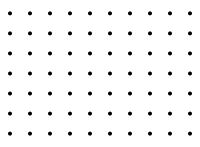
\includegraphics[width=3cm]{200px-SquareLattice}
    \label{fig:square-lattice}
  }
  \hspace{4mm}
  \subfloat[Parallelogram lattice.]{
    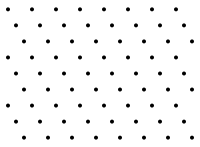
\includegraphics[width=3cm]{200px-Oblique_Lattice}
    \label{fig:lattice4}
  }
  \caption{Four simple lattice types in two dimensions.}
  \label{fig:lattices}
\end{figure}

Lattice noise is generated by having a lattice, and then for each
lattice point generating one or more random values for that point
depending on the type of noise we want.
%
The low-pass filtering is then done by interpolating the values at the
grid points to fill the entire space between the lattice
points. Different interpolation scheme can be used to calculate these
values, which yield different properties for the noise function.

\subsubsection{Value noise}
Value noise is the simplest type of lattice noise, here the values
stored at each grid point are the values that are interpolated and
returned when the function is evaluated.

\subsubsection{Gradient noise}
Gradient noise however generates a gradient at each point in the
lattice, which is a vector with the same dimensions as the number of
dimensions wherein the function is defined. The gradient in each grid
point is then used to calculate a continuous function between the grid
points, which again can be used to evaluate a noise value.
%
The gradient noise category includes the now famous noise
function known as Perlin noise, first described by Ken Perlin in
the paper: \citeabook{Perlin88}.
%
Here we once again want to warn the reader that many authors of web
pages,
e.g. \url{http://freespace.virgin.net/hugo.elias/models/m_perlin.htm},
seems to confuse Perlin noise with value noise, with the result that
an Internet search for Perlin noise becomes a non-trivial job. An
excellent describtion of Perlin noise can be found in
\citebook{chapter~12}{ebert2003} which is also written by Ken Perlin.

\section{Composition of layers}
Noise alone does not make realistic looking textures, only by carefully
choosing the noise parameters and cleverly combining many layers of
different looking noise results in natural beauty. In the following,
we will focus on generating a volumetric texture of clouds, but the
description illustrates the overall process of how to generate and
combine noise functions.
%
To describe how we combine noise functions, we will use terminology
borrowed from the field of digital signal processing, DSP. In DSP the
term \emph{sample frequency} describes the space between to
consecutive samples, and the term \emph{amplitude} the maximum value
of the function.

To generate the basic shape of some clouds we use a low
frequency noise with a large amplitude as illustrated for a one
dimensional case in figure in \ref{fig:1d-layer0}.
%
We add layers of details onto this low frequency noise by combining it 
with noise of higher frequencies.
%Where the details comes from the higher frequencies.
Because we want the basic shapes to be the most
dominant the amplitude of noise with higher frequencies are lowered,
this is shown in figure \ref{fig:1d-layer1} and \ref{fig:1d-layer2}.
%
We change these frequency and amplitude in octaves because octaves
frequently occur in nature and give good visual results.  For each
level of detail that is added, the frequency is doubled while the
amplitude is halved. To illustrate this, we have used value noise to
generate three layers and combined them into the result show in figure
\ref{fig:1d-result}.

\begin{figure}[!h]
  \centering
  \subfloat[Layer 0.]{
    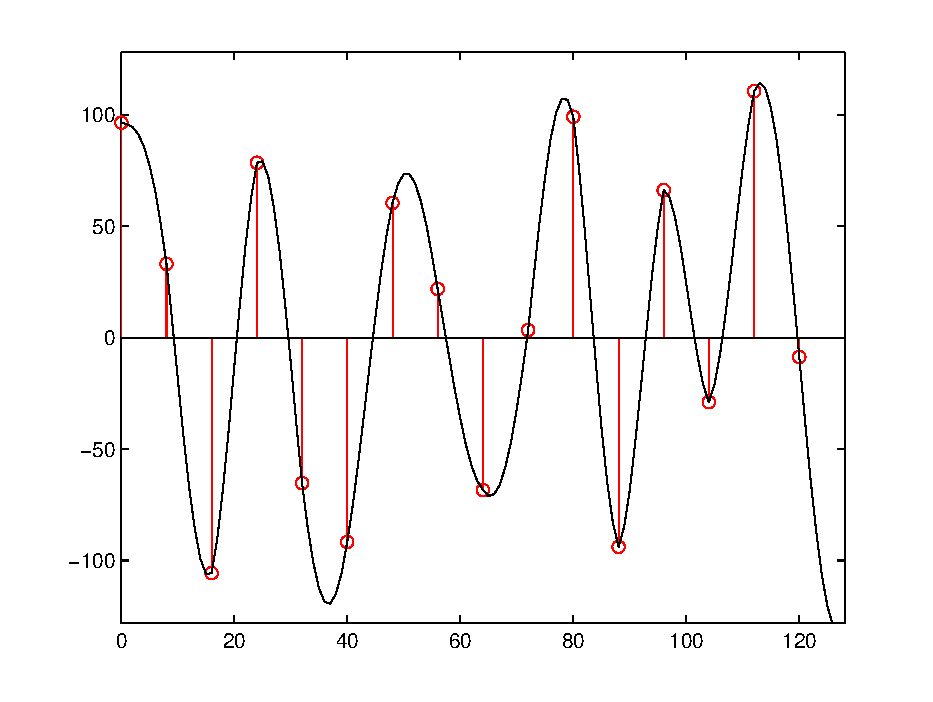
\includegraphics[width=7.25cm]{n0}
    \label{fig:1d-layer0}
  }
  \hspace{4mm}
  \subfloat[Layer 1.]{
    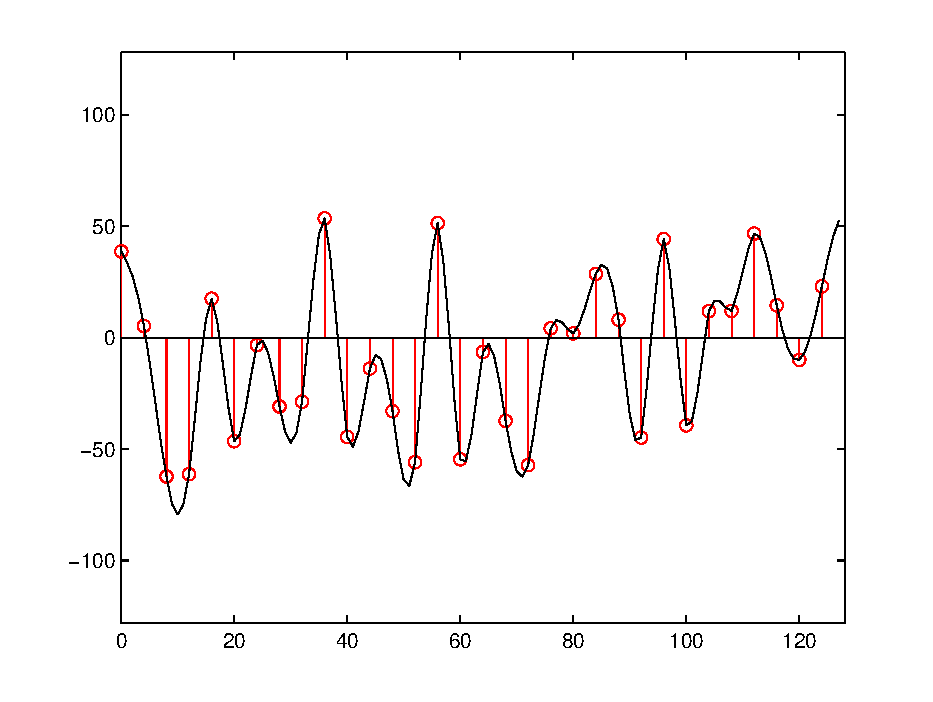
\includegraphics[width=7.25cm]{n1}
    \label{fig:1d-layer1}
  }
  \newline
  \centering
  \subfloat[Layer 2.]{
    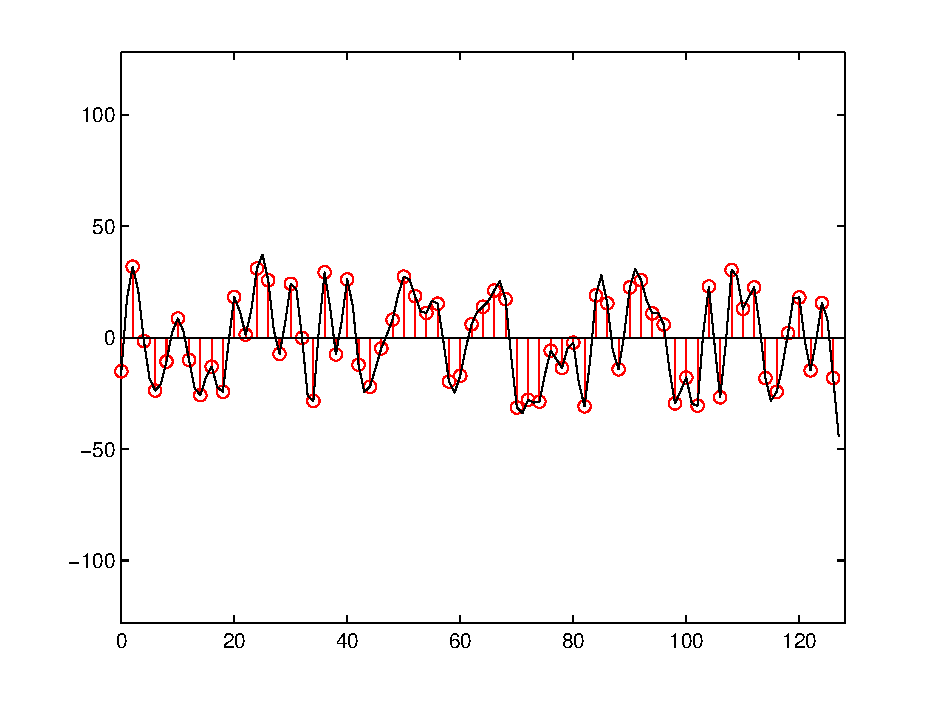
\includegraphics[width=7.25cm]{n2}
    \label{fig:1d-layer2}
  }
  \hspace{4mm}
  \subfloat[Result.]{
    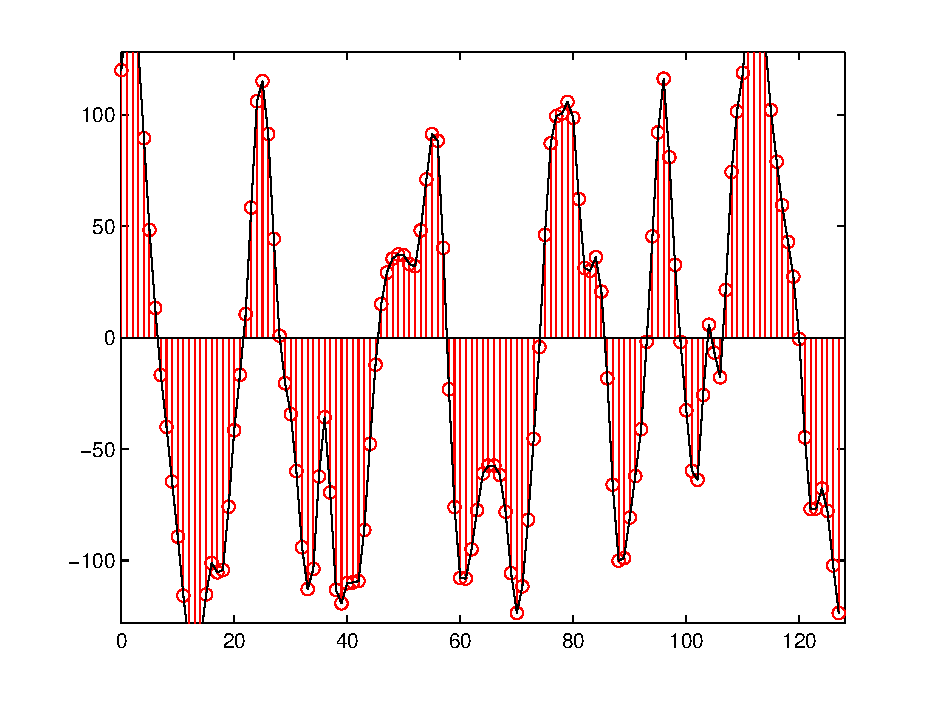
\includegraphics[width=7.25cm]{n0to2}
    \label{fig:1d-result}
  }
  \caption{One dimensional example of the combination process.}
  \label{fig:1d-layers}
\end{figure}

%\pagebreak
Moving into two and three dimensions are straight forward. Figure
\ref{fig:noise-layers} shows four layers of two dimensional white
noise rendered as alpha transparency on a fully white image, the blue
background has been inserted so the transparency can be seem. These
layers are the basic primitives for the upcoming combination into an
image that looks like clouds.
%
When sampling into an array, as has been done in figure
\ref{fig:noise-layers} the increase in sampling frequency is the same
as using a larger array. If this array represent an image or texture,
as in the figure, then the different layers do not have the same
height and width. To solve this, when algorithmically combining two
layers, the layer with the lowest resolution is re-sampled to the same
resolution as the other layer.

\begin{figure}[!h]
    \centering
    \subfloat[Layer 0.]{
      \colorbox{Cerulean} {
\includegraphics[width=3cm]{generated-rx8-b1024}}
      \label{fig:noise-layer0}
    }
  \hspace{4mm}
  \subfloat[Layer 1.]{
    \colorbox{Cerulean} {
\includegraphics[width=3cm]{generated-rx16-b512}}
    \label{fig:noise-layer1}
  }
  \hspace{4mm}
  \subfloat[Layer 2.]{
    \colorbox{Cerulean} {
\includegraphics[width=3cm]{generated-rx32-b256}}
    \label{fig:noise-layer2}
  }
  \hspace{4mm}
  \subfloat[Layer 3.]{
    \colorbox{Cerulean} {
\includegraphics[width=3cm]{generated-rx64-b128}}
    \label{fig:noise-layer3}
  }
  \caption{Four noise layers.}
  \label{fig:noise-layers}
\end{figure}

The layers are then combined two at the time. The process starts by
combining the two layers with lowest resolution. Then the result of
the previous combination is combined with the image with third lowest
resolution and so on.
%
Because we use linear interpolation between our lattice point, the
result of combining the layers, becomes very blocky looking, like the
image in figure \ref{fig:combined-layer1}. To get
around this we blur the result after each new layer is added, which
can be seem in figure \ref{fig:combined-layers}.

\begin{figure}[!h]
    \centering
    \subfloat[Combo of layer 0 to 1.]{
      \colorbox{Cerulean} {
\includegraphics[width=3cm]{combined-l1-b512}}
      \label{fig:combined-layer1}
    }
  \hspace{4mm}
  \subfloat[Combo of layer 0 to 2.]{
    \colorbox{Cerulean} {
\includegraphics[width=3cm]{combined-l2-b256}}
    \label{fig:combined-layer2}
  }
  \hspace{4mm}
  \subfloat[Combo of layer 0 to 3.]{
    \colorbox{Cerulean} {
\includegraphics[width=3cm]{combined-l3-b128}}
    \label{fig:combined-layer3}
  }
  \hspace{4mm}
  \subfloat[Result.]{
    \colorbox{Cerulean} {
\includegraphics[width=3cm]{output}}
    \label{fig:combined-result}
  }
  \caption{Snapshots of the combination process.}
  \label{fig:combined-layers}
\end{figure}

The final touch, after the image is generated, is to filter the image
with an exponential function which creates the look seen in figure
\ref{fig:combined-result}.

\section{Implementation}
When implementing noise functions, one must choose where the
computations are placed. One option is to do all computations as
pre-computations and then use the resulting noise texture for look up
at run-time. Another option is to do all the computations at
run-time. The main advantage of doing the calculation as pre-computation
is an increase in run-time performance, where as doing the calculations
at run-time enable dynamic adaption in LOD in relation to the camera
position. For the run-time computations to be fast enough for
real-time rendering they are usually done on the GPU, but although noise
functions exists in the GLSL API\citebook{page~145-146}{orangebook},
they are not recommended because
their behavior is not fully described in the specification and are
implemented differently by different vendors and on different
hardware. Developers that still want to do the calculations
at run-time, instead use a hybrid solution, generating a small noise
texture which can be used to implement more sophisticated noise
function on the GPU.
%
We however have chosen to do all the calculations as pre-computations
implemented for CPU execution. Our implementation is based the
\code{RandomGenerator} class of OpenEngine which again is based on the
PRN from \citebook{page~278-283}{NRIC2}.
%
The core of the entire algorithm for generating noise, composing
layers, and blurring them is implemented as the following recursive
function (the full implementation can be found in the \code{ValueNoise}
class of the \code{TexUtils} OpenEngine extension):

\begin{lstlisting}[frame=,language=C++]
    static FloatTexture2DPtr Generate(unsigned int xResolution, unsigned int yResolution,
                                      unsigned int bandwidth, float mResolution,
                                      float mBandwidth, unsigned int blur,
                                      unsigned int layers, RandomGenerator& r) {
            FloatTexture2DPtr noise =
                    CreateNoise(xResolution, yResolution, bandwidth, r.UniformInt(0,256));
            if (layers != 0) {
                FloatTexture2DPtr small = 
                    Generate(xResolution * mResolution, yResolution * mResolution, 
                             bandwidth * mBandwidth, mResolution, mBandwidth,
                             blur, layers-1, r);
                noise = Combine(noise, small);
                Blur(noise, blur);
            }
            return noise;
    }
\end{lstlisting}

%%% Local Variables:
%%% mode: latex
%%% TeX-master: t
%%% TeX-PDF-mode: t
%%% End:
